\section{Definition von SIEMs und Log Analysis Tools}

\gls{SIEM} ist das Ergebnis von der Kombination zwischen \glsfirst{SEM} und \glsfirst{SIM} \citep{Dorigo_SIEM}. Das erste bezieht sich auf der Identifizierung, Bewertung, Beobachtung und Bericht von Sicherheitsvorfällen mithilfe von verschiedenen Log Dateien \citep{techopedia_SEM}. Das zweite ist ein Software, der bei der automatischen Sammlung von Loginformationen aus vielen Quellen, wie Firewall und Servers, unterstützt \citep{techopedia_SIM}. Da die meisten \gls{SIEM} Lösungen kostenpflichtig sind, existieren auch viele \gls{Open Source} Log Analysis Tools die eine ähnliche Aufgabe erledigen, ohne die Kernelementen von \gls{SIEM}.

Log Analysis Tools sind meistens Anwendungen die Logdateien empfangen, speichern, bearbeiten und nach spezifisichen eigegenen Regeln bewerten. Diese Tools unterstützen Programmieren und Systemadministratoren bei der Überwachung des Zustands Systemen oder Software. Ein solches Tools kann Logdateien von verschiedenen \glsplural{Endpoint} und mit verschiedenen Formattierungen bekommen und editieren, so dass es schließlich ein Bericht oder Graphik erzeugt \citep{Korzeniowski_LATDef}. Die Nutzung dieser Tools schränkt sich nicht in dem Sicherheitsbereich ein, sondern kann für das gesamte Rechenzentren nützlich sein.

In dem Universum des \glsfirst{SOC} mischen sich verschiedene Begriffe, die manchmal zur Verwirrung führen, weil sie ähnliche Bedeutung und Verantwortung haben. \glsfirst{IDS}, \glsfirst{IPS}, \glsfirst{SIEM} und Log Analysis Tools werden von \textit{nonnative users} und sogar von Spezialisten oft verwechselt, da ihre Aufgabe mehr Zusammenhang als Unterschied haben. Um den Umfang dieser Arbeit wegen der zeitlichen Einschränkungen zu verringern, fassen wir kurz die Unterschiede zwischen ihnen zusammen und legen unsere Grenze auf den \glspl{SIEM} Lösungen und auf Log Analysis Tools fest.

\newpage
\glsfirst{IDS} sind Software oder Hardware, die \glsplural{Cyberangriff} identifizieren und berichten. Sie haben eine passive Rolle, weil sie die \glsplural{Cyberangriff}n weder stoppen noch verhindern können. \glsfirst{IPS} seinerseits haben eine aktive Haltung gegenüber \glsplural{Cyberangriff}, die können automatisch behandeln können, indem sie Blocking-Mechanism einschalten, um den Angriff zu stoppen \citep{Wendzel_IS}. Wie \gls{IDS}, kann der \gls{IPS} auch Logdateien generieren, die von einer \gls{SIEM} Lösung gesammelt werden können. \glsplural{SIEM} können seinerseits die Logdateien von diesen und von anderen \glsplural{Endpoint} bekommen und diese nach vordefierten Regeln bewerten, um dem \gls{SOC}-Team über Sicherheitsvorfälle zu informieren oder automatisch Maßnahmen zu greifen. Wie \glsplural{SIEM} bekommen Log Analysis Tools auch Logdateien, um Bericht oder Darstellung zu genieren, ihre Nutzung ist aber nicht so spezifisch wie von der \glsplural{SIEM}.

Die folgenden Abbildung stellt didaktisch eine allgemeine Struktur von \gls{SIEM}-Lösungen: 

\begin{figure}[H]
   \centering
   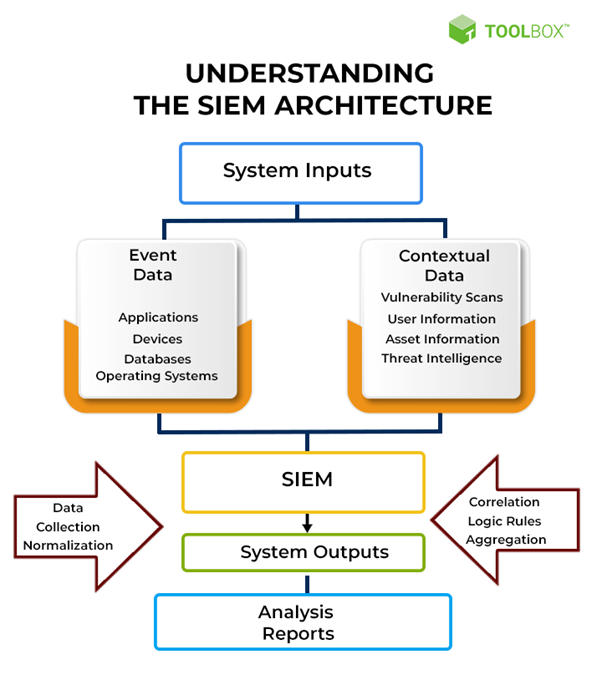
\includegraphics[width=0.5\textwidth]{assets/2_p1.png}
   \caption{Allgemeine Struktur von \gls{SIEM} \\Quelle: \citep{Mohanan_What} }
   \centering
\end{figure}

\newpage
Aus dem Bild können wir feststellen, dass \glsplural{SIEM} für die Zentralisierung von Sicherheitsdaten zuständig ist. Diese werden dann bearbeitet und in einem oder mehreren Berichten dargestellt, damit das \gls{SOC}-Team schnellere und effektive Entscheidungen treffen können. Der Informationsfluss einer \gls{SIEM} Lösung können wieder in der folgenden Abbildung darstellen:

\begin{figure}[H]
   \centering
   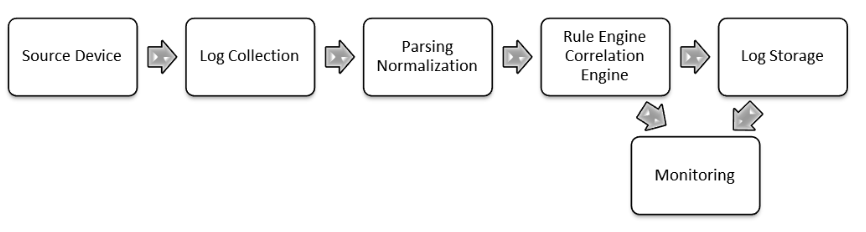
\includegraphics[width=0.8\textwidth]{assets/2_p2.png}
   \caption{Allgemeine Informationsfluss von \gls{SIEM} \\Quelle: \citep{Granadillo_SIEM} }
   \centering
\end{figure}

Die folgenden Abbildung stellen eine allgemeine Architektur von Log Analysis Tools dar:

\begin{figure}[H]
   \centering
   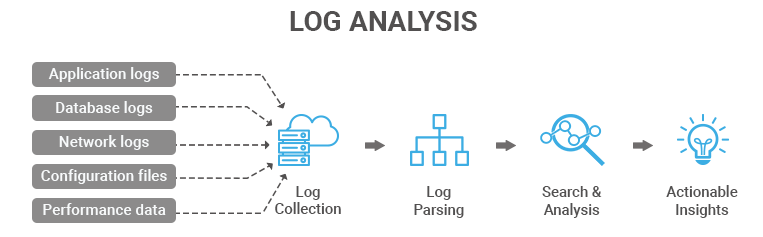
\includegraphics[width=0.8\textwidth]{assets/2.1_p2.png}
   \caption{Allgemeine Struktur von Log Analysys Tools\\Quelle: \citep{Tek-Tools_LGTArchitektur} }
   \centering
\end{figure}

\newpage
Den Informationsfluss eines Log Analysys Tools zeigen auf dem folgenden Bild:

\begin{figure}[H]
   \centering
   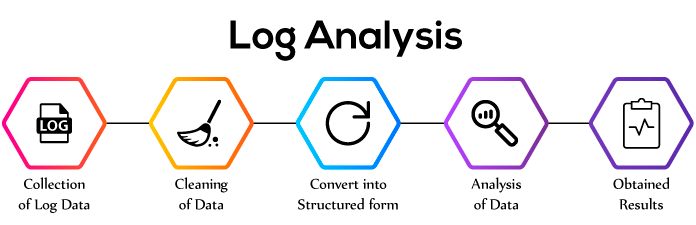
\includegraphics[width=0.8\textwidth]{assets/2.2_p2.png}
   \caption{Allgemeine Informationsfluss von Log Analysys Tools\\Quelle: \citep{Neptune_LATInfoFluss} }
   \centering
\end{figure}

Aus den bisherigen Beschreibung stellen wir fest, dass \gls{SIEM} viel mehr als eine Sammlung von Logdateien sind. Das Ziel dieser Software ist die automatische Analyse zu ermöglichen, indem Daten kombiniert und bewertet werden können. In vielen Bereiche, wie Finanzen (\glsfirst{PCDISS}), Gesundheitswesen (\glsfirst{HIPAA}), sind \glsplural{SIEM} gesetzliche Verpflichtung \citep{Jog_SIEM}. In Deutschland verplichtet das \gls{IT-Sicherheitsgesetz 2.0} Organisationen mit kritischen Infrastrukturen die Anwendungen von solche Lösungen, um Störungen der \glsfirst{CIA} zu verhindern \citep{BSI_ITSG}. Log Analysys Tools sind seinerseits allgemeine Tools zu der Speicherung, Anpassadung, Bewertung und Darstellung von Logdateien, ohne dass sie auf der Sicherheitsebenen fokussieren.




\subsection{Existierende SIEMs Lösungen und Log Analysis Tools }
% über Splunk schreiben, state of the art, nicht open source, aber andere müssen ähnliche funktionaliten haben
Die existierenden \glsplural{SIEM} Lösungen können in zwei Kategorien getrennt werden: \textit{\gls{Proprietary}} und \textit{\gls{Open Source}}. Zu der ersten ist Splunk von dem Unternehmen Splunk Technology, die zu der meist verwendeten Software \citep{Kazarov_Splunk} gehört und als \textit{State of the art} für andere \glsplural{SIEM} gilt. In den folgenden Abschnitte präsentiere wir Splunk, damit wir einen Maßtab für unsere Auswahl haben und demnächst und beschreiben wir folgenden \textit{\gls{Open Source}} Tools:

\begin{itemize}[noitemsep]
   \item Prelude
   \item AlienVault \glsfirst{OSSIM}
   \item FortiSIEM
   \item ELK Stack ++ Mittre ATT\&AT %(nein)
   \item Grafana
\end{itemize}

\textbf{\textcolor{red}{Wie konnte ich Grafana hier erwähnen? Grafane ist eher allgemein und nicht so zu Alert orientiert, habe ich hier gefunden: \href{https://www.metricfire.com/blog/grafana-vs-splunk/}{Splunk x Grafana} und hier \href{https://www.researchgate.net/publication/350730340_Implementation_of_Grafana_as_open_source_visualization_and_query_processing_platform_for_data_scientists_and_researchers}{What is Grafana}}  }

\subsubsection{Splunk}

bbbbbbbbbbbbbbbbbbb
% Regel von Mittre anhand einer SIEM Lösung an dem SIEM anpassen
% Grafana: 
% zeek: The Zeek Network Security Monitor => Tool ==> Verkehr umleiten und analysieren
% mittre: https://attack.mitre.org/
% https://socfortress.medium.com/part-6-best-open-source-siem-dashboards-5dad09fa4d0e
% Own SIEM: chrome-extension://efaidnbmnnnibpcajpcglclefindmkaj/http://prof.msoltys.com/wp-content/uploads/2019/02/Donnelly-Gittins.pdf



% 1 - zuerst Zugriffs auf Log von jeder anwendung
% 2 -  danach Zugriffs auf Log von Zeek Nehmen (Zeek) 

\subsubsection{Prelude}

% suche nach Modulen, die man separat benutzen kann (Correlator)
Das im Jahr 2002 in Frankreich von Yoann Vandoorselaere freigegebene Tool Prelude zählt zu gehört zu einer europäischen \gls{Open Source} \gls{SIEM} Lösung. Laut dem Anbieter verfügt Prelude unter anderen folgenden Funktionalitäten \citep{Prelude_SIEM}:

\begin{itemize}[noitemsep]
   \item Informations Zentralisierung 
   \item Datenaggregation und -Zusammenhang mit vordefinierten und von den Nutzer angepassten Regeln 
   \item Einbruchserkennungmechanismen
   \item Datennormalisierung
\end{itemize}

Die Anwendung besteht aus verschiedenen unabhängige Modulen. Unter denen highlighten wir folgende: Warnmeldung, Archivierung, Analyse und Verwaltung. Das erste gehört zu der zentralen Aufgabe dieser Lösung, es ist dafür zuständig, Daten zu empfangen, zu normalisieren, Zusammenhang zu machen und Meldungen zu generieren. Das zweite Modul, Archivierung, konzentriert sich auf die Speicherung und Verfügbarkeit der Daten. Zu der Analyse-Modul gehören statistische Aufgabe und Darstellung in verschiedenen Formaten. Das letzte Modul dient dazu, die Anwendung zu steuern, Nutzer zu erstellen dessen Rechts zu konfigurieren \citep{EC_Prelude}.

Die folgende Abbildung zeigt die Integration der verschiedenen Module von Prelude und wie sie sich kommunizieren, um Analyse, Meldung und Speicherung zu generieren:

\begin{figure}[H]
   \centering
   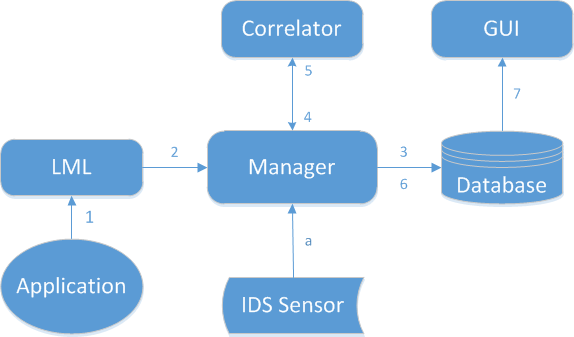
\includegraphics[width=0.8\textwidth]{assets/2_p3.png}
   \caption{Integration zwischen den Modulen von Prelude \\Quelle: \citep{Prelude_MU} }
   \centering
\end{figure}

Aus der Abbildung und der Dokumentation können wir folgenden Informationsfluss: die Daten werden von Endanwendung generiert und zum Loganalyzer (Prelude \glsfirst{LML}) geschickt, wo sie normalisiert und bewertet sind. Für solche Logs, wo es verdächtige Werte gibt, werden Warnmeldung generiert. Diese Meldung wird zum Manager Module weitergeleitet. Der Correlator oben sucht nach Zusammenhang zwischen andere Daten. Das Ergebnis von Correlator ist wieder zum Manager geschicht und danach zu der Datenbank. Schließlich stehen die Berichte in dem User-Interface zur Verfügung \citep{Prelude_Doc}.

Die Architektur der Anwendung ermöglicht sowohl einen zentralisierter als auch einen dezentralisierten Aufbau. In der nächsten Abbildung sehen wir eine einfache Implementation von Prelude: 

\begin{figure}[H]
   \centering
   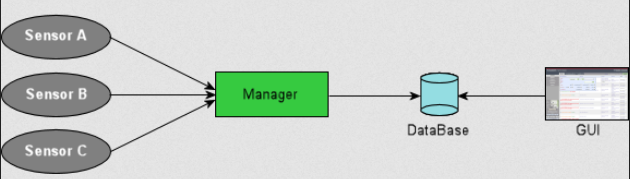
\includegraphics[width=0.8\textwidth]{assets/2_p4.png}
   \caption{Einfache Architektur von Prelude \\Quelle: \citep{Prelude_MU} }
   \centering
\end{figure}

In einer dezentralisierte Umgebung werden Daten von verschiedenen und getrennte Quellen generiert und bearbeitet. Schließlich können die Nutzer auf diesen Daten unter einem \gls{GUI} zugreifen.

\begin{figure}[H]
   \centering
   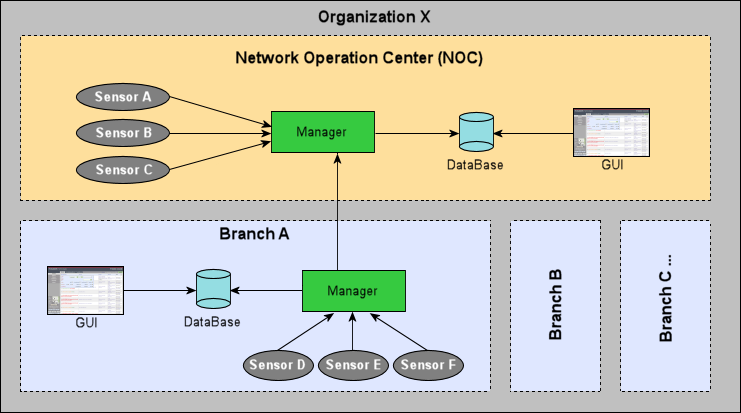
\includegraphics[width=0.8\textwidth]{assets/2_p5.png}
   \caption{Erweiterte Architektur von Prelude mit der Nutzung von dezentralisierten Datenquellen und Bearbeitung \\Quelle: \citep{Prelude_MU} }
   \centering
\end{figure}

Die wissenschaftliche Literatur über Prelude ist sehr eingeschränkt. Wenige Publikationen fokussieren sich auf die Entwicklung, Implementation und unternehmerische Anwendung dieses Tools. Eine Studie von 2021 versuchte dieses und zwei andere Tools (AlienVault und Cyberoam iView) anhand technischer und nutzerfreundliche Kriterien zu vergleichen. Unter diese Kriterien highlighten wir folgende \citep{Grammatikis_Prelude}:

\begin{itemize}[noitemsep]
   \item \textbf{technische Kriterien}
   \begin{itemize}[noitemsep]
      \item \textit{Real-time performance}, 
      \item \textit{Range and flexibility of reporting}
      \item \textit{Alert correlation}
   \end{itemize}

   \item \textbf{nutzerfreundliche Kriterien}
   \begin{itemize}[noitemsep]
      \item \textit{Documentation comprehensiveness}
      \item \textit{Complexity of the installation process}
      \item \textit{Complexity of the system configuration}
   \end{itemize}
\end{itemize}

In den technischen Kriterien lag Prelude auf dem dritten Platz und in den benutzerfreundlichen Kriterien bekam Prelude den ersten Platz. 

Auch in den nicht wissenschaftlichen Publikationen existiert eine begrenzte Anzahl von Texten über Preludes. Die existierenden kommentieren ganz zusammenfassend über die ausreichende Dokumentation und heben hervor, dass es eher eine in Europa konzentrierte Lösung ist.

\subsubsection{AlienVault OSSIM}
AlienVault OSSIM ist eine im Jahr 2007 entwickelte \gls{Open Source} SIEM Lösung. Im Jahr 2018 wurde sie von der Firma AT\&T Communication gekauft \citep{CBN_AV}. In der Beschreibung des Anbieters steht, dass sie auch dabei unterstützt, Daten zu sammeln, zu normalisieren und zu bewerten. Er behauptet auch, dass sein Tool in der Lage ist, Schwachstelle und Angriffe zu erkennen, Verhältnis zu beobachten und Daten Zusammenhang durchzuführen \citep{ATT_AVO}.

AlienVault hat eine kostenpflichtige Version, die Alien Vault \glsfirst{USM} heißt. In der Webseite von AT\&T steht, dass es keine spezifische Dokumentation für die \gls{Open Source} Version, AlienVault OSSIM, gibt, weil viele Funktionalitäten von der anderen Version stammen \citep{ATT_AVO}. 

Die folgende Abbildung zeigt das von dem Anbieter freigelegte Architekturdiagramm von der \gls{USM} Version:

\begin{figure}[H]
   \centering
   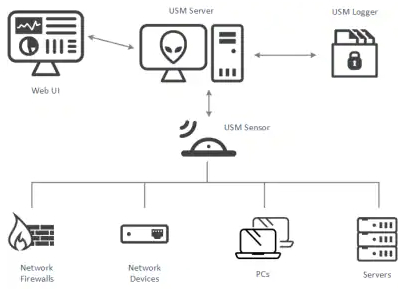
\includegraphics[width=0.6\textwidth]{assets/2_p6.png}
   \caption{Architekturdiagramm  ram von AlienVault \gls{USM} \\Quelle: \citep{ATT_AVO} }
   \centering
\end{figure}

Laut der Website Comparitech steht AlienVault in der 13ten Platz von den besten bewerteten \gls{SIEM} Lösungen. Die Seite beschreibt auch, dass einen \gls{IDS}, Verhaltensüberwachungssystem und einen Schwachstellen-Scanner integriert sind . Die Anwendung ist auch mit der Platform \gls{OTX} verbunden, diese ermöglicht die Teilung von Informationen über Schwachstelle. Comparitech highlighted, dass die Anwendung wegeren ihre niedrigen Kosten besser für kleine oder mittelständige Unternehmen geeignet ist \citep{comparitech_SIEM}. 

Die Anwendung soll konsistenten Daten Zusammenhang anbieten und soll das Auftauchen von \gls{falsch positiv} vermeiden. AlienVault kommt auch mit vordefinierten Use-Cases, die dabei unterstützen gewöhnlichen Angriffsszenario zu erkennen. Die Installation, die Einstellung und die Integration mit anderen Tools ist auch benutzerfreundlich \citep{Gomes_AV}. Aus einer anderen wissenschaftlichen Quelle fanden wir heraus, dass für viele  Quelle eine manuelle Normalisierung der Logdatein notwendig ist \cite{Nabil_AV}. Die Anwendung hat aber einen zuverlässigen Berichtsmechanismus.

Während unserer Recherche gab es wenig wissenschaftliche Literatur, die sich um AlienVault OSSIM kümmert. Kommerzielle Publikationen waren auch viel auf die Firma AT\&T auf die kostenpflichtige Version des Tools konzentriert.

\subsubsection{FortiSIEM}
FortiSIEM ist eine US-amerikanische \gls{SIEM} Lösung von der Firma Fortinet. Fortinet kaufte im Jahr 2016 das Unternehmen AccelOps und dessen \gls{SIEM} Lösung und benannte es zum FortSIEM \citep{Fortinet_Press}. 

Laut dem Anbieter hat FortiSIEM eine robuste Integration mit anderen Tools und lässt sich leicht und einwandfrei skalieren. Andere Versionen des Tools sind mit Machine Learning integriert, sodass die Anwendung auch Verhältnisanalyse durchführen kann \citep{Fortinet_Solutions}. Das Tool bietet auch eine umfangreiche und ausführliche Dokumentation an. Die nächste Abbildung zeigt die skalierbare Architektur des Tools:

\begin{figure}[H]
   \centering
   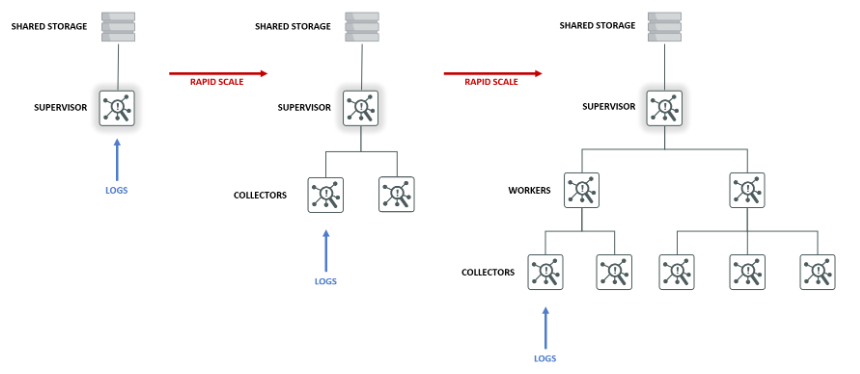
\includegraphics[width=1\textwidth]{assets/2_p7.png}
   \caption{Skalierbare Architektur von FortiSIEM \\Quelle: \citep{Fortinet_Arch} }
   \centering
\end{figure}

Auch zu dieser \gls{SIEM} Lösung ist die wissenschaftliche Produktion eingeschränkt. Eine von der gefundenen Publikation betont, dass FortiSIEM eine schnelle Erkennung von Angriffen  anbietet und über \glsfirst{NOC} Funktionalitäten verfügt \citep{Ramires_fortisiem}. Wie andere \glspl{SIEM} Lösungen hat FortiSIEM folgende Funktionalitäten:

\begin{itemize}[noitemsep]
   \item Datensammlung und Normalisierung
   \item Daten Zusammenhang
   \item Generierung von Berichten
   \item Warnmeldungen
   \item Datenauswertung 
\end{itemize}

\subsubsection{ELK Stack}
ELK Stack stammt aus der Verbindung von drei ürsprüngliche \gls{Open Source} Tools: Elasticsearch, Logstash und Kibana. Das erste ist eine Such- und Analyse-Maschine. Das zweite ist eine Serverseitige Anwendung zur Datenverarbeitung und -Weiterleitung. Schließlich Kibana ist dafür zuständig, visuelle Darstellung in Grafik-Format auszugeben \citep{packt_elkstack}. Dieses Tool besitzt viele Eigenschaften von einer \gls{SIEM}-Lösung und ist von vielen \gls{SOC} verwendet, ist aber, für viele Experten, kein \gls{SIEM} für sich, da es über keine Warnmeldungssystem, Daten Zusammenhang und Vorfälleverwaltung verfügt \citep{Miller_ELK}. Diese und anderen Funktionalitäten lassen sich aber durch \glsplural{plugin} integrieren. 

Das folgende Diagramm stellt die Architektur von ELK Stack mit ihren integrierten Elementen  dar:

\begin{figure}[H]
   \centering
   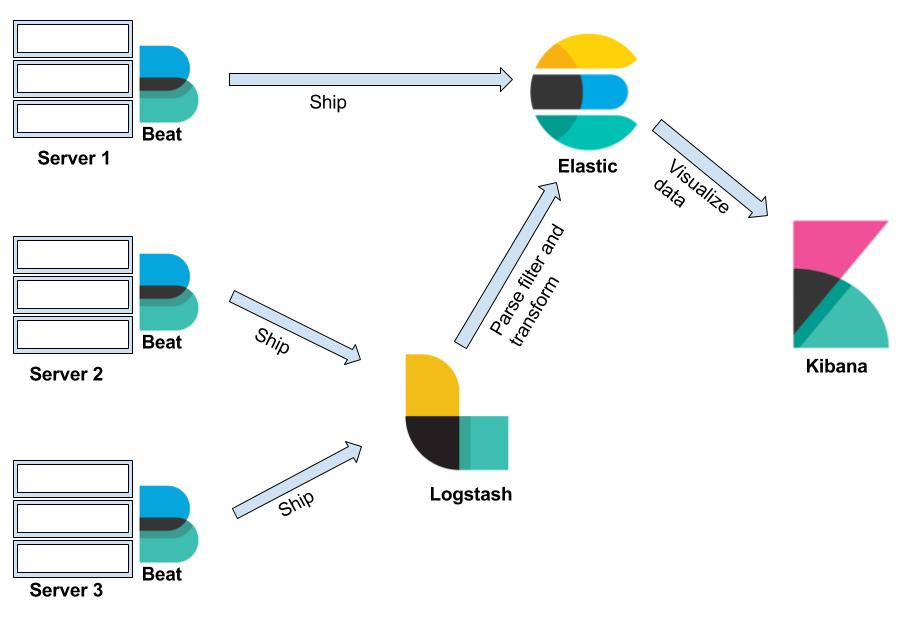
\includegraphics[width=0.8\textwidth]{assets/2_p8.png}
   \caption{Integration zwischen Elasticsearch, Logstash und Kibana\\Quelle: \citep{packt_elkstack} }
   \centering
\end{figure}

Auf dem Bild werden auch Beats gezeigt. Diese Komponenten sind an der Endanwendung installiert und sie leiten Daten entweder zu Elasticsearch oder zu Logstash weiter, wo sie schließlich bearbeitet werden \citep{Jain_LMELK}. 

Ein Teil der wissenschaftlichen Literatur zeigt die Log Analyse-Funktionalitäten von ELK Stack und die Unterstützung bei Normalisierung und Indexierung von Daten für eine lesbare Ausgabe \citep{Advani_elkstakc}. Die starke Skalierbarkeit wurde auch bei einer Studie erwähnt, wo ELK Stack für Wi-Fi Logging eingesetzt wurde wurde \citep{Wang_elkwifi}.

Die offiziele Dokumentation von ELK Stack betont, dass die Anwendung folgende Funktionalitäten besitzen:  mit der Anwendung folgendes möglich ist \citep{elastic_docs}:

\begin{itemize}[noitemsep]
   \item Datensuche, -Normalisierung, -Analyse und 
   \item Speicherung
   \item visuelle Ausgabe
\end{itemize}

Folgendes Diagramm aus der offiziellen Dokumentation zeigt die Aufteilung der Funktionalitäten por Element von ELK Stack:

\begin{figure}[H]
   \centering
   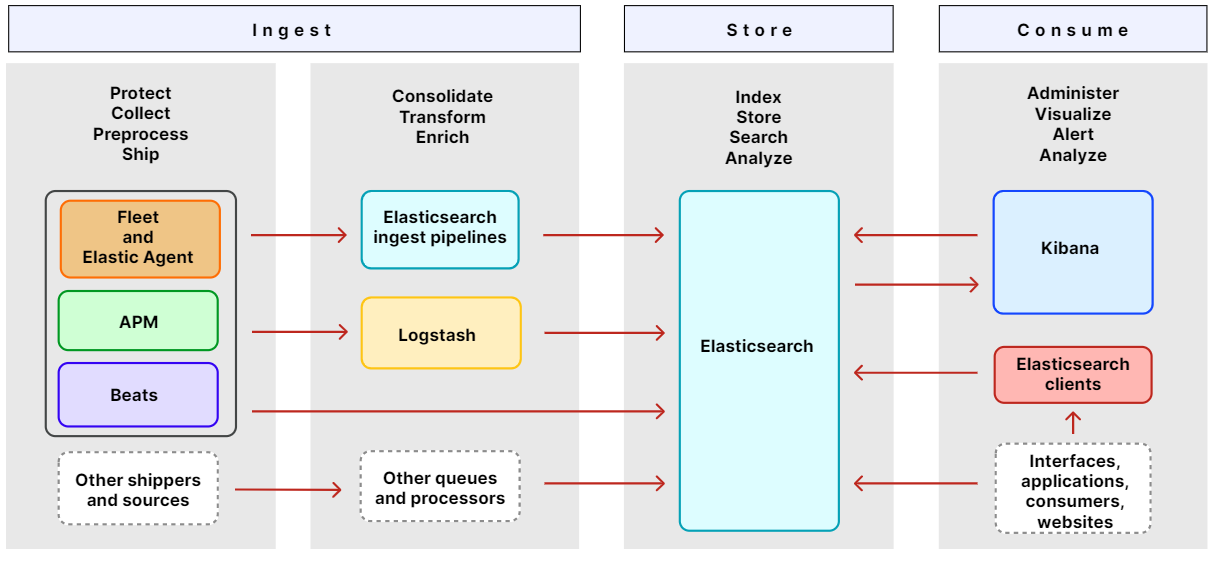
\includegraphics[width=0.8\textwidth]{assets/2_p9.png}
   \caption{Aufteilung der Funktionalitäten zwischen den Komponenten\\Quelle: \citep{elastic_docs}}
   \centering
\end{figure}

Die wissenschaftliche Publikation über ELK Stack ist vielfältiger als bei der anderen recherchierten Tools. Es ist aber wichtig, zu betonen, dass die Mehrheit von denen sich eher mit dem Logging als mit den \gls{SIEM}-Eingeschaften der Anwendung beschäftigt.

\subsubsection{Grafana}
AAAAAAAAAAAAAAAAAAAAAAAA


\subsection{Auswahlkrietieren}
Die wichtigste Kriteria für unsere Auswahl war, dass die Anwendung \gls{Open Source} sein sollte. Kostenpflichtige Versionen können wegen ihrem Preis und Komplexität besonders kleinere Unternehmen abschrecken und infolgedessen bleiben sie fern von einigen Sicherheitslösungen \citep{Bjork_OSSIEM}.

Für diese haben entschieden wir uns für die XXXXX \gls{SIEM} Lösung aus folgenden Grunden:

\begin{itemize}[noitemsep]
   \item eingeschränkte Ressource für die Entwicklung dieser Arbeit
   \item bbbbbbbbbbbbbbb
   \item ccccccccccccccc
   \item ddddddddddddddd
   \item eeeeeeeeeeeeeee
\end{itemize}

Demnächst fokussieren wir uns auf dieInstallation, Konfiguration und Implementation von XXXXXX. Danach werden wir spezifische Logdateien der Hochschule importieren, normalisieren und diese anhand Angriff1 und Angriff2 beobachten.